{\bf BME154L - Spring 2012 - Exam \#2 Solutions}\hfill Name (Net ID):\underline{\hspace*{3.0in}}



\vspace*{0.5in}

\centerline{\LARGE BME154L (Palmeri)}
\vspace*{0.25in}
\centerline{\LARGE Spring 2012}
\vspace*{0.25in}
\centerline{\LARGE Exam \#1}
\vspace*{0.25in}

{\bf Instructions:} 
\begin{itemize}
\item Write your name at the top of each page.
\item Show all work (this is {\it critical} for partial credit!).
\item \underline{Remember to include units with all answers and label all plot axes.}
\item Clearly box all answers.
\item Assume that all components are ideal unless otherwise stated.
\item Assume that op amps rail at $\pm$ 12 V unless otherwise stated.
\end{itemize}

\begin{center}
\begin{tabular}{cc}
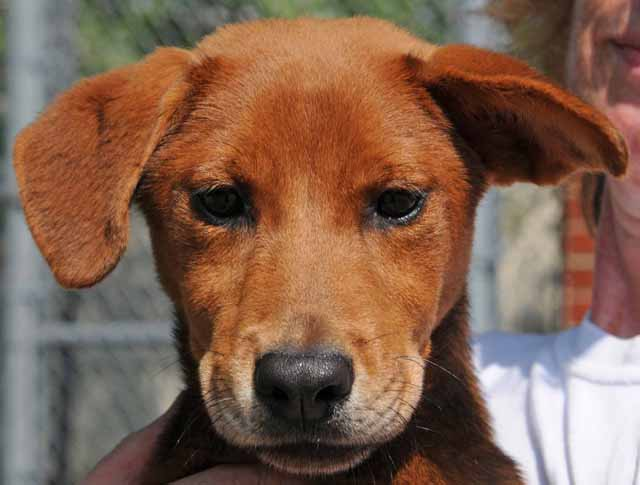
\includegraphics[width=0.39\linewidth]{avery.jpg} &
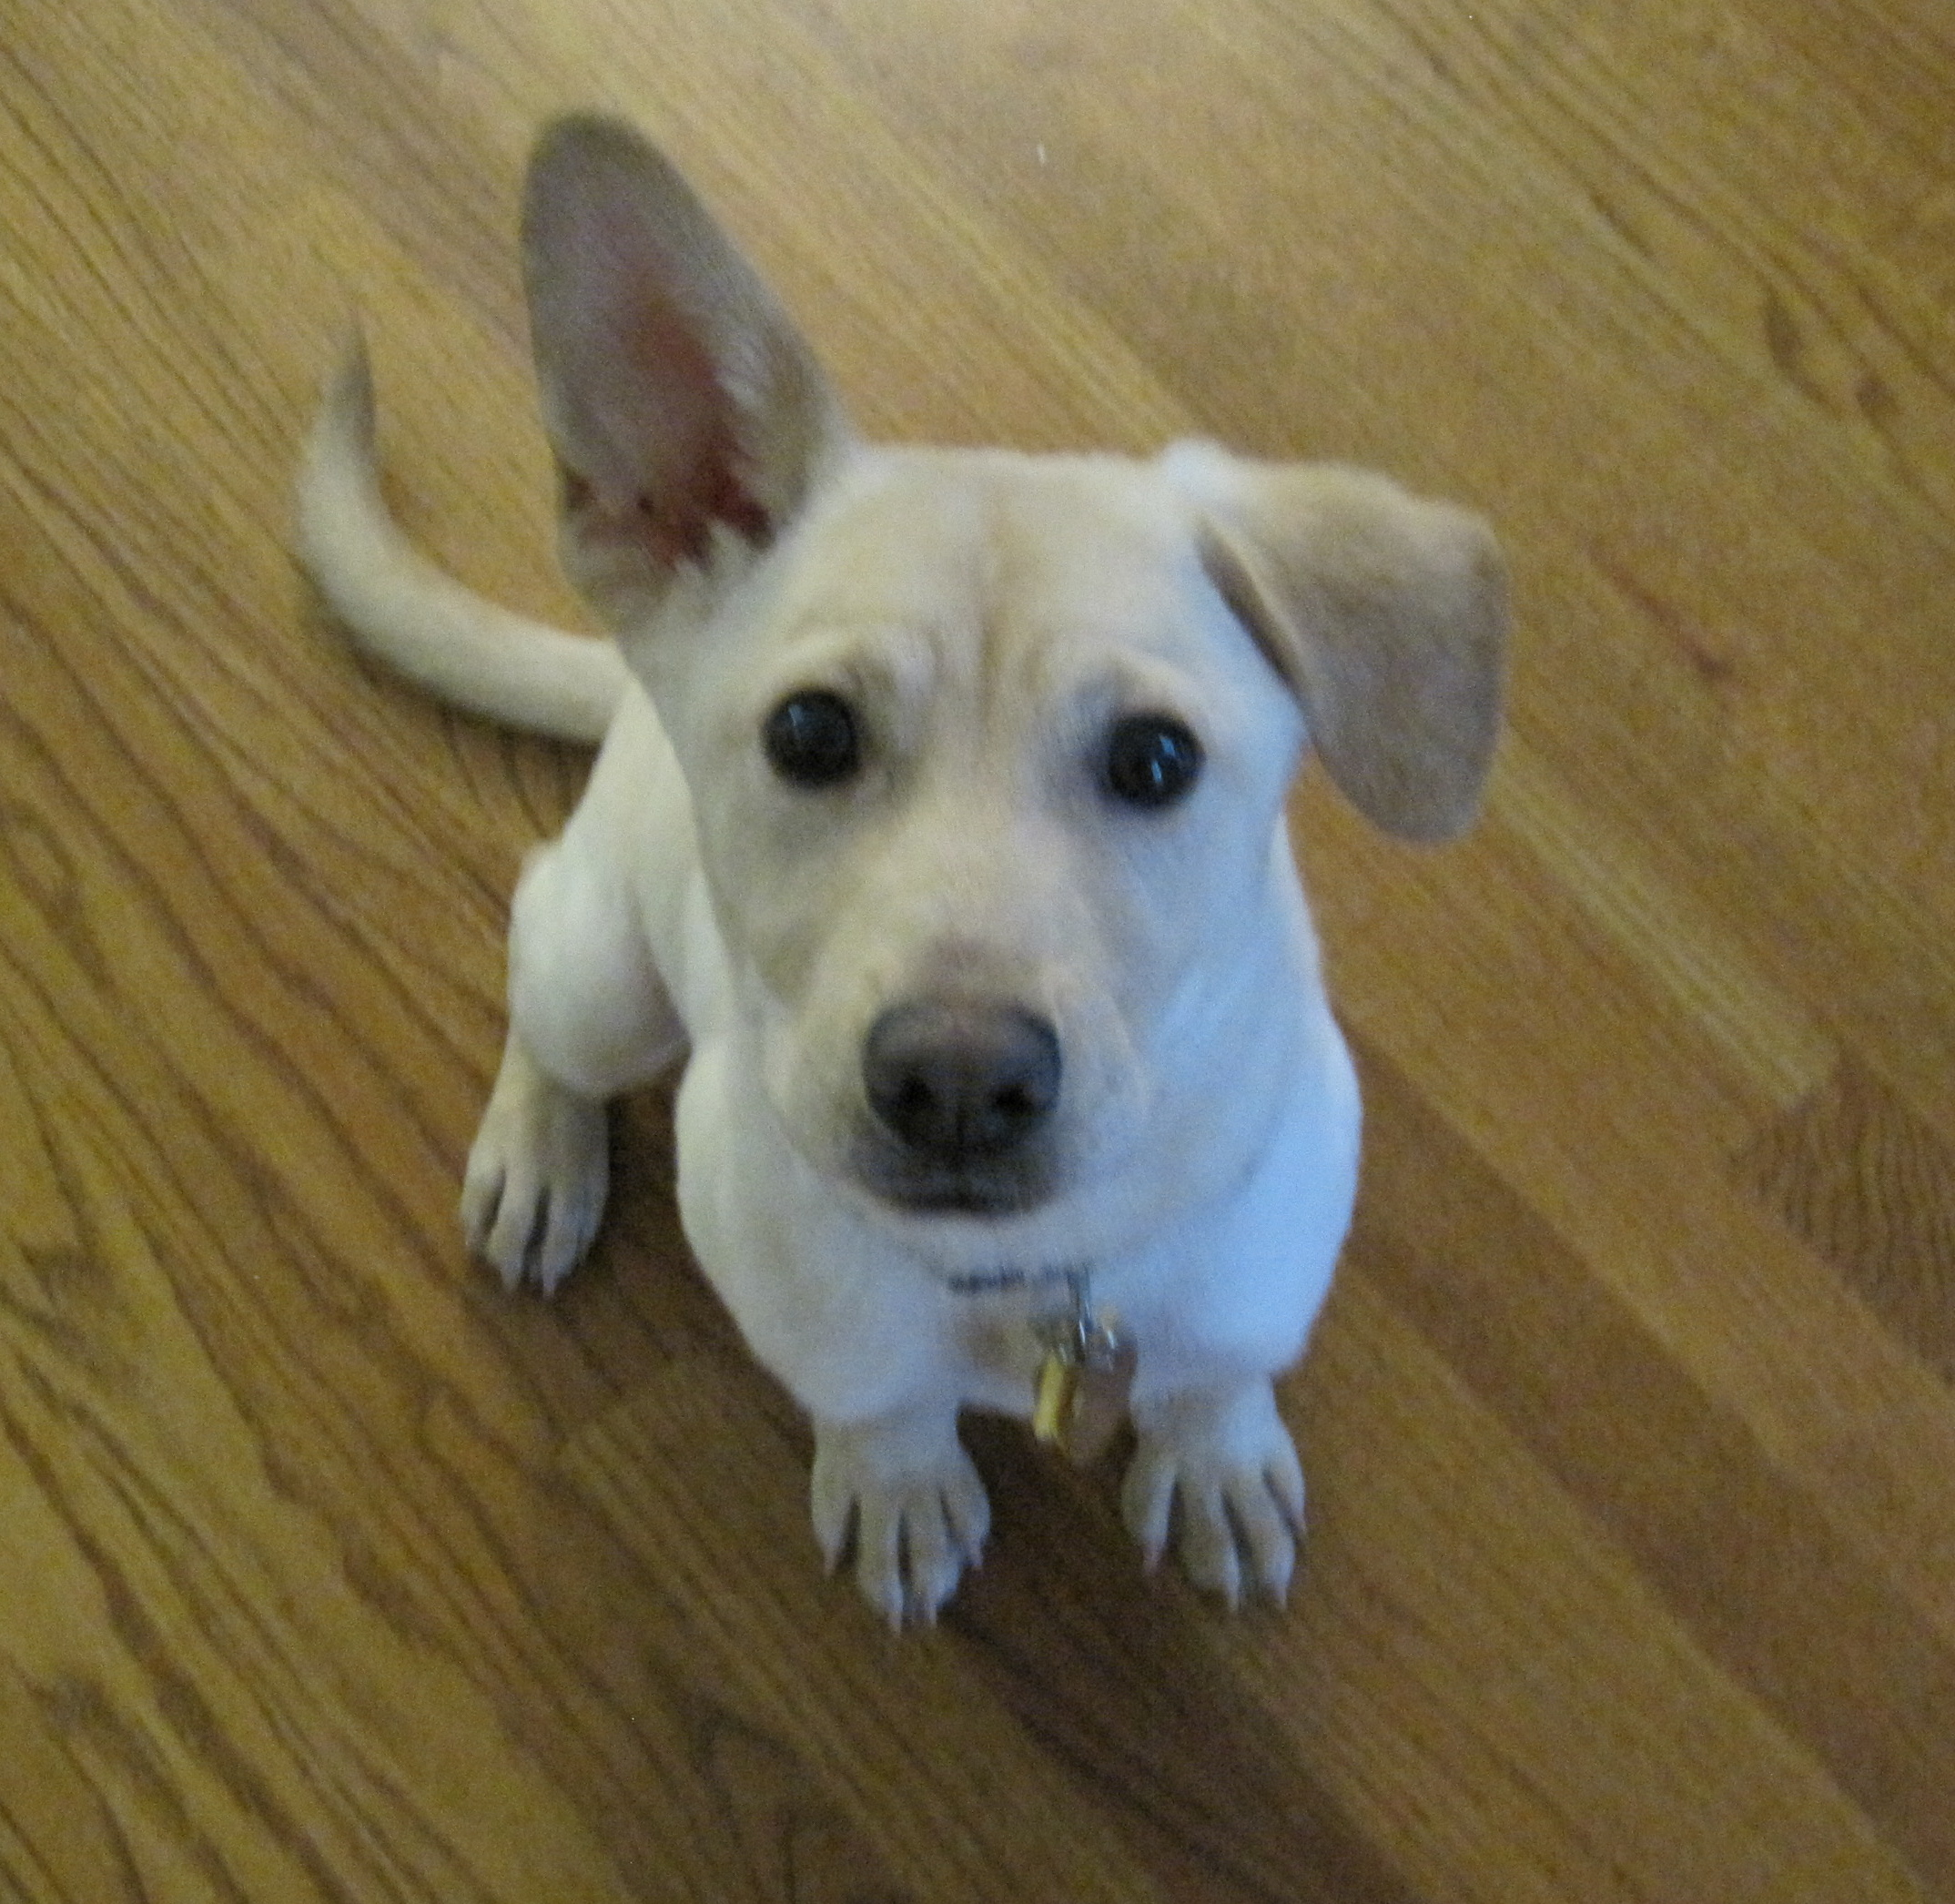
\includegraphics[width=0.3\linewidth]{ziva.jpg} \\
\end{tabular}

Avery \& Ziva wish you good luck!!
\end{center}


\emph{In keeping with the Duke Community Standard, I have neither given nor received aid in completion of this examination.}

\vspace*{0.5in}

Signature:\underline{\hspace*{3.0in}}
